\documentclass[a4paper,12pt]{article}

\usepackage{graphicx} % Required for inserting images
\usepackage{amsmath,amssymb,amsfonts}
\usepackage{subcaption}
% Use Times New Roman font
\usepackage{times}
\usepackage[a4paper, top=1in, bottom=0.8in, left=1.1in, right=0.8in]{geometry}
\usepackage{float}
\usepackage{listings}
\usepackage{xcolor} % For customizing code colors
\setlength{\parindent}{0pt}

\begin{document}
	
	\section{Experiment No. 2}
	\section{Experiment Title }
Measurement of Inductance by using Wattmeter, Ammeter \& Voltmeter.
	\section{Objective}
	The objectives of this lab are as follows:
	\begin{itemize}
		\item To determine the inductance of a electrical inductor using Wattmeter,Ammeter \& Voltmeter.
		\item To know the proper connection method of Wattmeter across a load.
	\end{itemize}
	
	\section{Theory}
	
	Inductance (\( L \)) is a property of an electrical circuit that opposes changes in current. It is often measured using an ammeter, voltmeter, and wattmeter. For an AC circuit containing an inductor, the voltage (\( V \)) and current (\( I \)) are out of phase due to the inductive reactance (\( X_L \)), which is directly proportional to the frequency (\( f \)) of the AC signal. The total impedance (\( Z \)) of the circuit is the combination of the inductor's reactance and any resistive components present in the circuit.
	
	The power (\( W \)) measured by the wattmeter is the true power consumed by the resistive part of the circuit, while the reactive power is associated with the inductor. By knowing the current, voltage, and power, we can calculate the following parameters:
	
	\begin{itemize}
		\item \textbf{Resistance (\( R \))}: The resistance of the circuit can be calculated from the power and the current using the equation:
		\[
		R = \frac{W}{I^2}
		\]
		where \( W \) is the power measured by the wattmeter and \( I \) is the current measured by the ammeter.
		
		\item \textbf{Impedance (\( Z \))}: The total impedance of the circuit can be calculated using Ohm's law:
		\[
		Z = \frac{V}{I}
		\]
		where \( V \) is the voltage measured by the voltmeter and \( I \) is the current measured by the ammeter.
		
		\item \textbf{Reactance (\( X_L \))}: The inductive reactance of the circuit can be found by subtracting the resistive component from the total impedance:
		\[
		X_L = \sqrt{Z^2 - R^2}
		\]
		where \( Z \) is the total impedance and \( R \) is the resistance calculated earlier.
		
		\item \textbf{Inductance (\( L \))}: Finally, the inductance of the coil can be determined from the reactance and the frequency of the AC signal:
		\[
		L = \frac{X_L}{2 \pi f}
		\]
		where \( X_L \) is the inductive reactance and \( f \) is the frequency of the AC signal, which is typically 50 Hz.
	\end{itemize}
	
	In this experiment, we connect the wattmeter to measure the power consumed by the resistive part of the circuit, and using the above equations, we can determine the inductance of the inductor. The reactance is derived from the measured impedance and resistance, and the inductance is calculated from the reactance.
	
	\section{Required Apparatus}
	\begin{enumerate}
		\item Wattmeter(0-240V,0-10A),
		\item Voltmeter(0-450V),
		\item Ammeter(0-1A),
		\item Inductor(1.26 H),
		\item Variac(0-250V),
		\item AC power supply(230V, 50 Hz),
		\item Connecting Wire.

	\end{enumerate}
	\section{Circuit Diagram}
	\begin{figure}[H]
		\centering
		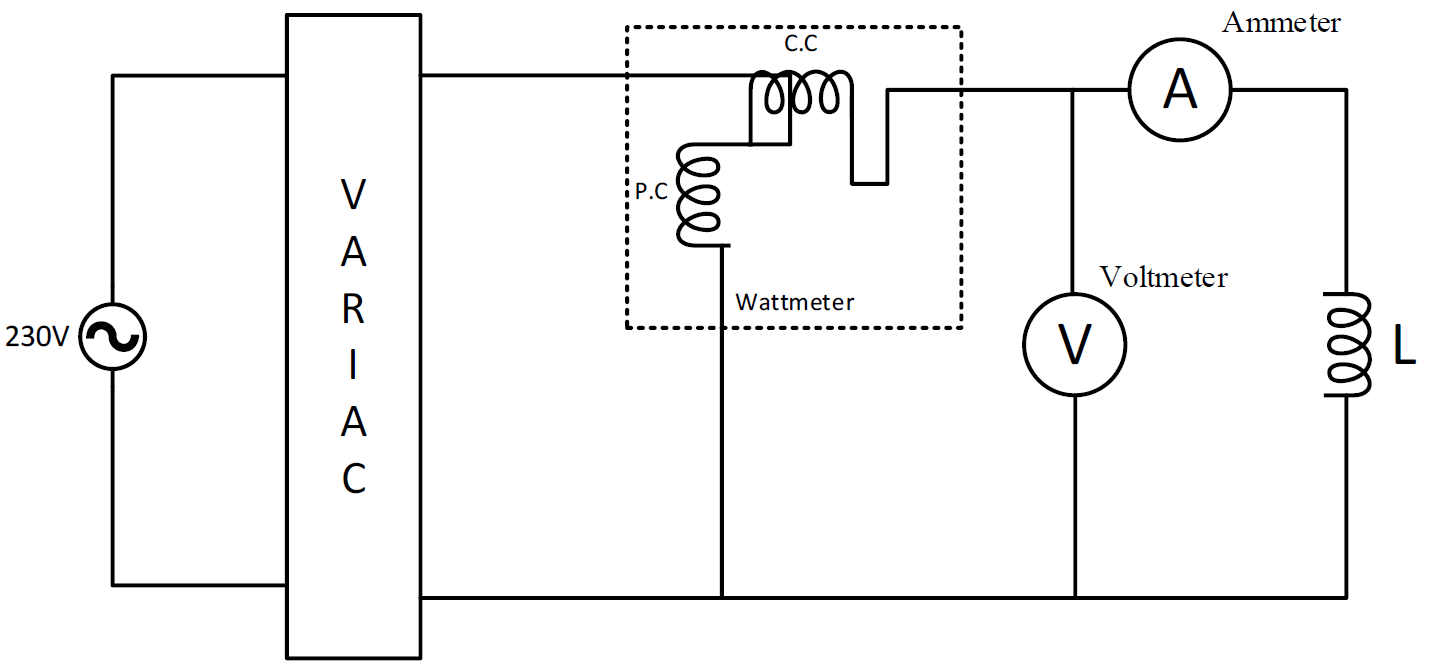
\includegraphics[width=1\linewidth]{Images/1.4}
		\caption{Circuit diagram for measurement of inductance}
		\label{fig:1}
	\end{figure}
	\newpage
	\section{Data Table}
	
	\begin{table}[H]
		\resizebox{\textwidth}{!}{
			\begin{tabular}{|l|c|c|c|c|c|c|c|}
				\hline
				\multicolumn{1}{|c|}{\textbf{\begin{tabular}[c]{@{}c@{}}No\\ of\\ Obs.\end{tabular}}} & \textbf{\begin{tabular}[c]{@{}c@{}}Voltmeter\\ Reading\\ (V)\end{tabular}} & \textbf{\begin{tabular}[c]{@{}c@{}}Ammeter\\ Reading\\ (A)\end{tabular}} & \textbf{\begin{tabular}[c]{@{}c@{}}Wattmeter\\ Reading\\ (W)\end{tabular}} & \textbf{\begin{tabular}[c]{@{}c@{}}Resistance\\ $ R = \frac{W}{I^{2}}$ \\ ($\Omega$)\end{tabular}} & \textbf{\begin{tabular}[c]{@{}c@{}}Impedance\\ $ Z = \frac{V}{I} $ \\ ($\Omega$)\end{tabular}} & \textbf{\begin{tabular}[c]{@{}c@{}}Reactance\\ $ X_L = \sqrt{Z^{2}-R^{2}} $ \\ ($\Omega$)\end{tabular}} & \textbf{\begin{tabular}[c]{@{}c@{}}Inductance\\ $ L = \frac{X_L}{2 \pi f}$ \\ (H)\end{tabular}} \\ \hline
				1. & 100 & 0.2 & 2 & 50 & 502 & 499.5 & 1.589 \\ \hline
				2. & 150 & 0.45 & 4.4 & 21.72 & 333.33 & 332.6 & 1.058 \\ \hline
				3. & 200 & 0.625 & 7 & 17.92 & 526.31 & 319.49 & 1.017 \\ \hline
			\end{tabular}
		}
	\end{table}
	
	\section{Calculation}
	
	The following calculations were performed for each observation to determine the electrical parameters: Resistance (\( R \)), Impedance (\( Z \)), Reactance (\( X_L \)), and Inductance (\( L \)). The frequency of the circuit was maintained at \( f = 50\,\text{Hz} \).
	
	\begin{enumerate}
		\item 
		For  \( V = 100\,\text{V} \) , \( I = 0.2\,\text{A} \),   \( W = 2\,\text{W} \) and   \( f = 50\,\text{Hz} \)
		
		
		
		\begin{enumerate}
			
			\item 
			\[
			X_L = \sqrt{Z^{2} - R^{2}} = \sqrt{500^{2} - 50^{2}} = \sqrt{250000 - 2500} = \sqrt{247500} \approx 497.5\,\Omega
			\]
			\item
			\[
			L_1 = \frac{X_L}{2\pi f} = \frac{497.5\,\Omega}{2\pi \times 50\,\text{Hz}} \approx \frac{497.5}{314.16} \approx 1.589\,\text{H}
			\]
			
			
		\end{enumerate}
		
		\item 	
		
		for \( V = 150\,\text{V} \)
		, \( I = 0.45\,\text{A} \)
		\, \( W = 4.4\,\text{W} \)
		and \( f = 50\,\text{Hz} \)
		
		
		\begin{enumerate}
			
			\item 
			\[
			X_L = \sqrt{Z^{2} - R^{2}} = \sqrt{333.33^{2} - 21.72^{2}} \approx \sqrt{110639.33} \approx 332.6\,\Omega
			\]
			\item
			\[
			L_2 = \frac{X_L}{2\pi f} = \frac{332.6\,\Omega}{2\pi \times 50\,\text{Hz}} \approx \frac{332.6}{314.16} \approx 1.058\,\text{H}
			\]
			
		\end{enumerate}
		
		
		\item 
		
		
		For	\( V = 200\,\text{V} \)
		, \( I = 0.625\,\text{A} \)
		, \( W = 7\,\text{W} \)
		and \( f = 50\,\text{Hz} \)
		
		\begin{enumerate}
			
			\item 
			\[
			X_L = \sqrt{Z^{2} - R^{2}} = \sqrt{320^{2} - 17.92^{2}}  \approx \sqrt{102078.8736} \approx 319.49\,\Omega
			\]
			\item
			\[
			L_3 = \frac{X_L}{2\pi f} = \frac{319.49\,\Omega}{2\pi \times 50\,\text{Hz}} \approx \frac{319.49}{314.16} \approx 1.017\,\text{H}
			\]
			
			
		\end{enumerate}
		
	\end{enumerate}
	\subsection{Average Inductance}
	\[ \bar{L} = \frac{L_1 + L_2 + L_3}{3} = 1.22\,\text{H} \]
	
	\section{Result}
	The average inductance is \( \bar{L} = 1.22\,\text{H} \).
	

	\section{Discussion}
	
	In this experiment, the inductance of an inductor was determined using the measurements of voltage, current, and power and it was $1.22$H The wattmeter was used to measure the power consumed by the resistive component of the circuit. The resistance (\( R \)) was calculated using the formula \( R = \frac{W}{I^2} \), where the power and current were recorded during the experiment.
	
	The total impedance (\( Z \)) was obtained by dividing the measured voltage by the current, using \( Z = \frac{V}{I} \). This provided the overall opposition to the AC current in the circuit, which included both the resistive and inductive effects.
	
	From the calculated impedance and resistance, the inductive reactance (\( X_L \)) was computed using the formula \( X_L = \sqrt{Z^2 - R^2} \). This allowed the contribution of the inductive component to be isolated from the total impedance.
	
	Finally, the inductance (\( L \)) of the inductor was found by dividing the inductive reactance by \( 2\pi f \), where \( f \) was the frequency of the AC power supply. The average inductance was then calculated from the individual values obtained from each set of measurements. The results demonstrated that the inductance remained relatively consistent across different voltage and current values, confirming the accuracy of the method.
	
%	\[
%	R = \frac{W}{I^{2}}\,(\Omega), \quad
%	Z = \frac{V}{I}\,(\Omega), \quad
%	X_L = \sqrt{Z^{2} - R^{2}}, \quad
%	L = \frac{X}{2 \pi f}\,\text{(H)}
%	\]
	
\end{document}
